\documentclass{article}
\usepackage[zh]{homework}
\usepackage{tikz}
\usetikzlibrary{arrows.meta}
% 题目及原作业说明忠实转录自 HW5.pdf; 以下承诺要求为原文件内容.

\config{Algebra-1}{2026 秋季}{5}

\begin{document}

{\heiti 我承诺, 本次作业的完成没有使用大语言模型.}


\paragraph{约定} 群作用均为左作用. $N\unlhd G$ 表示 $N$ 是 $G$ 的正规子群. 复合 $g\circ f$ 表示先做 $f$, 再做 $g$, 置换乘积也从右向左作用. $\mathbf{Set}$, $\mathbf{Grp}$ 分别表示集合与函数, 群与群同态组成的范畴. 所涉及的范畴均假设局部小, 指标范畴均为小范畴, 函子均为协变函子; 允许使用选择公理.

本次作业共 10 题, 第 1--8 题必做, 第 9, 10 题选做.

可使用课堂已证明的结果及此前必做题的结论, 但不得将当前小问要求证明的结论作为已知结果直接引用.

\section*{习题}

\begin{problem}
设 $f,g:A\to B$ 是范畴 $\mathcal C$ 中具有相同源和靶的两个态射. 它们的等化子 (equalizer) 是满足 $f\circ e=g\circ e$ 的态射 $e:E\to A$, 且具有如下泛性质: 对任意满足 $f\circ u=g\circ u$ 的态射 $u:T\to A$, 存在唯一态射 $\overline u:T\to E$, 使 $e\circ\overline u=u$. 等价地, $E$ 连同映射 $e:E\to A$, $f\circ e:E\to B$, 是图 $A\rightrightarrows B$ 的极限.
\begin{enumerate}
  \item[(a)] 对群同态 $f,g:A\to B$, 证明
  \[
    E=\{a\in A:f(a)=g(a)\}
  \]
  是 $A$ 的子群, 且包含映射 $E\hookrightarrow A$ 是 $f,g$ 在 $\mathbf{Grp}$ 中的等化子. 由此说明, $\ker f\hookrightarrow A$ 是 $f$ 与平凡同态 $A\to B$ 的等化子; 这里平凡同态将每个元素送到 $B$ 的单位元.
  \item[(b)] 取 $A=B=S_3$, $f=\operatorname{id}_{S_3}$, $g=c_{(12)}$, 其中 $c_{(12)}(\sigma)=(12)\sigma(12)^{-1}$. 求出 $E$ 的所有元素, 并证明 $E$ 不是 $S_3$ 的正规子群.
\end{enumerate}
\end{problem}

\begin{solution}
	\paragraph{(a)} 先来证明 $E \le A$. 事实上, 由于 $f(1_A) = g(1_A) = 1_B$, 因此 $1_A \in E$; 对于 $x \in E$, 由 $f(x^{-1}) = f(x)^{-1} = g(x)^{-1} = g(x^{-1}	)$ 知 $x^{-1} \in E$; 对于 $x, y \in E$, 由 $f(xy) = f(x)f(y) = g(x)g(y) = g(xy)$ 知 $xy \in E$. 因此 $E \le A$. 

	再来证明 $E \hookrightarrow A$ 是 $f,g$ 在 $\mathbf{Grp}$ 中的等化子. 记上面的嵌入映射为 $\iota$. 则根据 $E$ 的定义, 有 $f \circ \iota = g \circ \iota$. 并且, 对于任意的群同态 $u: T \to A$ 满足 $f \circ u = g \circ u$, 对任意的 $t \in T$, 有 $f(u(t)) = g(u(t))$, 因此 $u(t) \in E$. 取 $\bar{u} = u$, 知 $u = \iota \circ \bar{u}$, 并且由 $\id_A|_{E} = \iota$ 不难知道这样的 $\bar{u}$ 是唯一的. 因此 $\iota$ 是等化子.

	记平凡同态为 $e$. 则有 $E = \{a \in A: f(a) = e(a) = 1_{B}\} = \ker f$. 因此 $\ker f \hookrightarrow A$ 为 $f$ 和 $e$ 的等化子. 

	\paragraph{(b)} 经过计算, 知 $E = \{(1), (12)\}$. 由于 $(13)E(13)^{-1} = \{(1), (23)\} \neq E$, 因此 $E$ 不是 $S_3$ 的正规子群.
\end{solution}



\begin{problem}
设 $f,g:A\to B$ 是范畴 $\mathcal C$ 中具有相同源和靶的两个态射. 它们的余等化子 (coequalizer) 是满足 $q\circ f=q\circ g$ 的态射 $q:B\to Q$, 且具有如下泛性质: 对任意满足 $v\circ f=v\circ g$ 的态射 $v:B\to T$, 存在唯一态射 $\overline v:Q\to T$, 使 $\overline v\circ q=v$. 等价地, $Q$ 连同映射 $q\circ f:A\to Q$, $q:B\to Q$, 是图 $A\rightrightarrows B$ 的余极限.

对群 $B$ 的子集 $S$, 记 $\langle\!\langle S\rangle\!\rangle_B$ 为包含 $S$ 的最小正规子群, 称为 $S$ 在 $B$ 中的正规闭包 (normal closure).
\begin{enumerate}
  \item[(a)] 对群同态 $f,g:A\to B$, 证明
  \[
    N=\big\langle\!\big\langle\{f(a)g(a)^{-1}:a\in A\}\big\rangle\!\big\rangle_B.
  \]
  且商映射 $q:B\to B/N$ 是 $f,g$ 在 $\mathbf{Grp}$ 中的余等化子.
  \item[(b)] 设 $H\le G$, 考虑包含同态与平凡同态 $H\rightrightarrows G$. 确定它们的余等化子. 当 $H\unlhd G$ 时, 结果如何简化? 当 $G=S_3$, $H=\langle(12)\rangle$ 时, 具体求出这个余等化子.
\end{enumerate}
\end{problem}

\begin{solution}
	\paragraph{(a)} 先来证明 $q \circ f = q \circ g$, 这是因为, 对于任意的 $a \in A$, 由于 $f(a)g(a)^{-1} \in N$, 因此 $q(f(a)g(a)^{-1}) = 1_{B/N}$, 故 $q(f(a)) = q(g(a))$, 即 $q \circ f = q \circ g$. 

	再来证明泛性质. 对于任意满足 $v \circ f = v \circ g$ 的同态 $v: B \to T$, 对任意的 $a \in A$, 有
	\[ v(f(a)g(a)^{-1}) = v(f(a))v(g(a))^{-1} = 1_T. \]
	因此 $\ker v$ 包含所有的 $f(a)g(a)^{-1}$. 又由于 $\ker v \unlhd B$, 故由正规闭包的定义知 $N \subseteq \ker v$. 若 $b_1N = b_2N$, 则 $b_2^{-1}b_1 \in N \subseteq \ker v$, 因此 $v(b_1) = v(b_2)$. 故映射
	\[ \bar{v}: \ B/N \to T, \ bN \mapsto v(b). \]
	是良定义的. 并且, 对于任意的 $b_1, b_2 \in B$, 有
	\[ \bar{v}((b_1N)(b_2N)) = v(b_1b_2) = v(b_1)v(b_2) = \bar{v}(b_1N)\bar{v}(b_2N), \]
	因此 $\bar{v}$ 是群同态.

	对于任意的 $b \in B$, 有 $v(b) = \bar{v}(bN) = \bar{v} \circ q(b)$, 因此 $v = \bar{v} \circ q$. 若存在两个同态 $\bar{v}_1, \bar{v}_2$ 满足 $v = \bar{v}_1 \circ q = \bar{v}_2 \circ q$, 由于 $q$ 是满射, 因此是 $\mathbf{Grp}$ 中的满态射, 故 $\bar{v}_1 = \bar{v}_2$. 因此 $q$ 是余等化子.

	\paragraph{(b)} 设包含同态为 $\iota$, 平凡同态为 $e$. 则余等化子为商映射 $G \to G/\braket{\!\braket{H}\!}$. 若 $H \unlhd G$, 则余等化子为上映射 $G \to G/H$. 如果 $G = S_3$, $H = \braket{(12)}$, 则 $\braket{\!\braket{H}\!} = G$, 因此余等化子为平凡同态 $G \to G/G \cong \{1\}$.
\end{solution}



\begin{problem}
设范畴 $\mathcal C$ 中任意两个对象的积及任意一对平行态射的等化子都存在. 给定态射 $f:A\to C$, $g:B\to C$, 记积的投影为 $\pi_A:A\times B\to A$, $\pi_B:A\times B\to B$.
\begin{enumerate}
  \item[(a)] 设 $e:P\to A\times B$ 是 $f\circ\pi_A,g\circ\pi_B:A\times B\rightrightarrows C$ 的等化子. 证明 $P$ 连同 $\pi_A\circ e$, $\pi_B\circ e$ 是 $f,g$ 的拉回 (pullback or fiber product 课上讲过).
  \item[(b)] 由此证明: 对群同态 $f:A\to C$, $g:B\to C$, 子群
  \[
    A\times_C B=\{(a,b)\in A\times B:f(a)=g(b)\}
  \]
  连同两个坐标投影, 是 $f,g$ 在 $\mathbf{Grp}$ 中的拉回.
\end{enumerate}
\end{problem}

\begin{solution}
	\paragraph{(a)} 令 $p_A = \pi_A \circ e$, $p_B = \pi_B \circ e$. 由 $e$ 是等化子, 知
	\[ f \circ p_A = (f \circ \pi_A) \circ e = (g \circ \pi_B) \circ e = g \circ p_B. \]
	而对于任意的态射 $u: T \to A$ 和 $v: T \to B$ 满足 $f \circ u = g \circ v$, 由 $A \times B$ 的泛性质, 知存在唯一的 $h: T \to A \times B$, 满足 $\pi_A \circ h = u$, $\pi_B \circ h = v$. 由于 $e$ 是 $f \circ \pi_A$ 与 $g \circ \pi_B$ 的等化子, 因此对于 $h$, 存在唯一的态射 $\bar{h}: T \to P$, 满足 $e \circ \bar{h} = h$. 此时, 
	\[ p_A \circ \bar{h} = \pi_A \circ e \circ \bar{h} = \pi_A \circ h = u, \]
	同理 $p_B \circ \bar{h} = v$. 因此我们证明了拉回所满足的相容性与泛性质, 故 $P$ 连通 $p_A, p_B$ 是 $f, g$ 的拉回.

	\paragraph{(b)} 熟知 $Z(G) \le G$. 我们只需要证明嵌入映射 $e: A \times_C B \hookrightarrow A \times B$ 是 $p_A := f \circ \pi_A$, $p_B := g \circ \pi_B$ 的等化子. 事实上, 由 $A \times_C B$ 的定义, 显然有 
	\[ p_A \circ e = f \circ (\pi_A \circ e) = g \circ (\pi_B \circ e) = p_B \circ e. \]

	并且, 对于任意的同态 $h: T \to A \times B$ 满足 $p_A \circ h = p_B \circ h$, 考虑同态
	\[ \bar{h}: \ T \to A \times_C B, t \mapsto h(t). \]
	由于对于任意的 $t \in T$, 由于 $f \circ (\pi_A \circ h) = p_A \circ h = p_B \circ h = g \circ (\pi_B \circ h)$, 故 $h(t) \in A \times_C B$, 即 $\bar{h}$ 是良定义的. $\bar{h}$ 显然满足 $e \circ \bar{h} = h$. 并且, 由于 $e$ 是嵌入映射, 因而是单射, 因此满足上述条件的 $\bar{h}$ 是唯一的. 故 $A \times_C B$ 连同两个坐标投影是 $f, g$ 在 $\mathbf{Grp}$ 中的拉回.
\end{solution}



\begin{problem}
对群 $G$, 记 $\mathbf BG$ 为对应的单对象群胚, 唯一对象为 $*$, 将 $\Hom_{\mathbf BG}(*,*)$ 与 $G$ 识别, 并规定 $g\circ h=gh$. 对 $s\in G$, 记 $c_s:G\to G$ 为共轭自同构 $c_s(x)=sxs^{-1}$. 考虑
\[
  D_G:\mathbf BG\longrightarrow\mathbf{Grp},\qquad D_G(*)=G,\qquad D_G(g)=c_g.
\]
\begin{enumerate}
  \item[(a)] 验证 $D_G$ 是函子. 证明群
  \[
    Z(G)=\{x\in G:xg=gx\text{ 对所有 }g\in G\text{ 成立}\}
  \]
  连同包含映射 $Z(G)\hookrightarrow G$, 是 $D_G$ 的极限, 从而得到 $\lim_{\mathbf BG}D_G\cong Z(G)$.
  \item[(b)] 设 $H\le G$, 沿包含函子 $\mathbf BH\to\mathbf BG$ 限制 $D_G$. 证明所得图的极限由
  \[
    C_G(H)=\{x\in G:xh=hx\text{ 对所有 }h\in H\text{ 成立}\}
  \]
  及其到 $G$ 的包含映射给出. 这里 $C_G(H)$ 称为 $H$ 在 $G$ 中的中心化子 (centralizer), 不假设 $H$ 正规.
\end{enumerate}
\end{problem}

\begin{solution}
	\paragraph{(a)} 先来验证 $D_G$ 是函子. 由于 $D_G(\id_{*}^{\mathbf{B}G}) = c_{1_G} = \id_G^{\mathbf{Grp}}$, 并且对于 $g_1, g_2 \in \Aut_{\mathbf{B}G}(*)$, 有 $D_G(g_1 \circ g_2) = c_{g_1g_2} = c_{g_1} \circ c_{g_2} = D_G(g_1) \circ D_G(g_2)$, 因此 $D_G$ 是函子.

	再来验证 $Z(G)$ 连同 $Z(G) \hookrightarrow G$ 是 $D_G$ 的极限. 由于 $\mathbf{B}G$ 只有一个元素, 因此可以将两个函子 $F_{1,2}: \mathbf{B}G \to \mathbf{Grp}$ 之间的自然变换视作 $F_{1,2}(*_{\mathbf{B}G})$ 之间的态射. 事实上, 对于任意的群 $H$ 以及可以被视为自然变换的态射 $f: H \to G$, 定义映射 
	\[ \bar{f}: H \to Z(G), h \mapsto f(h). \]
	我们只需证明 $\bar{f}$ 良定义且唯一. 

	任取 $g \in \Aut(*_{\mathbf{B}G})$, 由于 $\Delta_H(g) = \id_H$, $D(G)(g) = c_g$, 因此根据自然变换的定义, 有 $f \circ \id_H = c_g \circ f$, 即 $f = c_g \circ f$. 由此知, 对于任意的 $h \in H$, 以及任意的 $g \in G$, 均有 $f(h) = c_g(f(h)) = g f(h) g^{-1}$, 因此 $g f(h) = f(h) g$. 由 $g$ 的任意性, 知 $f(h) \in Z(G)$. 所以 $\bar{f}$ 是良定义的. 

	并且, 由于嵌入映射 $\iota: Z(G) \hookrightarrow G$ 是单射, 因此满足 $\iota \circ \bar{f} = f$ 的映射 $\bar{f}$ 是唯一的. 

	综上, 我们证明了 $Z(G)$ 连通 $\iota: Z(G) \hookrightarrow G$ 是 $D_G$ 的极限, 因此 $\lim_{\mathbf{B}G}D_G \cong Z(G)$. 

	\paragraph{(b)} 设限制 $D_G$ 得到的函子为
	\[ F: \ \mathbf{B}H \to \mathbf{Grp}, \ *_{\mathbf{B}H} \mapsto G, \ h \in \Aut(*) \mapsto c_h \in \Aut(G). \]
	与 (a) 同理, 只需将共轭元素的范围从 $G$ 限制为 $H$. 首先, $1_G \in C_G(H)$, 且对于任意的 $x, y \in C_G(H)$ 以及 $h \in H$, 有
	\[ c_h(xy^{-1}) = c_h(x)c_h(y)^{-1} = xy^{-1}. \]
	因此 $C_G(H) \le G$. 记嵌入映射为 $\iota: C_G(H) \hookrightarrow G$. 对于任意的 $h \in H$, 由中心化子的定义知 $c_h \circ \iota = \iota$, 因此 $\iota$ 给出了 $F$ 的一个锥.

	对于任意的群 $K$ 以及锥 $u: K \to G$, 有 $c_h \circ u = u$ 对所有的 $h \in H$ 成立. 因此对于任意的 $k \in K$ 和 $h \in H$, 有 $hu(k)h^{-1} = u(k)$, 即 $hu(k) = u(k)h$, 故 $u(k) \in C_G(H)$. 于是同态
	\[ \bar{u}: \ K \to C_G(H), k \mapsto u(k) \]
	是良定义的, 并且满足 $\iota \circ \bar{u} = u$. 由于 $\iota$ 是单射, 因此满足上述条件的 $\bar{u}$ 是唯一的. 综上, $C_G(H)$ 连同嵌入映射 $\iota$ 是 $F$ 的极限.
\end{solution}



\begin{problem}
沿用第 4 题的函子 $D_G:\mathbf BG\to\mathbf{Grp}$. 定义
\[
  [g,x]=gxg^{-1}x^{-1},\qquad [G,G]=\langle[g,x]:g,x\in G\rangle,
\]
即 $[G,G]$ 是由所有交换子 $[g,x]$ 生成的子群, 称为交换子子群 (commutator subgroup).
\begin{enumerate}
  \item[(a)] 证明 $[G,G]\unlhd G$, 且 $G/[G,G]$ 是阿贝尔群.
  \item[(b)] 证明 $G/[G,G]$ 连同商映射
  \[
    q:G\longrightarrow G/[G,G]
  \]
  是 $D_G$ 在 $\mathbf{Grp}$ 中的余极限. 具体地, 验证 $q\circ c_g=q$ 对所有 $g\in G$ 成立; 并证明, 对任意群 $K$ 及满足 $u\circ c_g=u$ (对所有 $g\in G$) 的同态 $u:G\to K$, 存在唯一同态 $\overline u:G/[G,G]\to K$, 使 $\overline u\circ q=u$.
  \item[(c)] 计算 $\operatorname{colim}_{\mathbf BS_3}D_{S_3}$. 设 $U:\mathbf{Grp}\to\mathbf{Set}$ 为遗忘群结构, 只保留底层集合与映射的函子. 再计算 $\operatorname{colim}_{\mathbf BS_3}(U\circ D_{S_3})$ 在 $\mathbf{Set}$ 中的结果, 并比较它与 $U(\operatorname{colim}_{\mathbf BS_3}D_{S_3})$ 的元素个数.
\end{enumerate}
\end{problem}

\begin{solution}
	\paragraph{(a)} 先证明 $[G,G] \unlhd G$. 这是因为, 对于任意的 $[g_1, g_2] \in [G, G]$ 与 $g \in G$, 有
	\[ g[g_1, g_2]g^{-1} = gg_1g_2g_1^{-1}g_2^{-1}g^{-1} = [gg_1g^{-1}, gg_2g^{-1}] \in [G, G]. \]
	因此 $[G, G] \unlhd G$. 

	再来证明 $G/[G, G]$ 是阿贝尔群. 对于 $a_1 = g_1[G, G]$ 和 $a_2 = g_2[G, G]$, 有
	\[ a_1a_2a_1^{-1}a_2^{-1} = g_1g_2g_1^{-1}g_2^{-1}[G, G] = [G, G] = \id_{G/[G, G]}. \]
	因此 $G/[G, G]$ 是阿贝尔群.

	\paragraph{(b)} 记 $A := G/[G, G]$. 与第 4 题类似, 我们将从 $\mathbf{B}G$ 出发的两个函子之间的自然变换看做一个态射. 对于任意的群 $H$, 取 $D_G$ 与 $\Delta_H$ 之间的一个自然变换, 并且设其对应的群同态为 $f$. 我们只需要证明: 存在唯一的自然同构 $\Delta_A \Rightarrow \Delta_H$, 其对应群同态 $\bar{f}: A \to H$, 满足 $f = \bar{f} \circ q$. 

	先来证明 $q$ 对应一个自然变换 $D_G \Rightarrow \Delta_A$. 对于任意的 $x, g \in G$, 有 $q(x) = q(x[x^{-1}, g]) = q(gxg^{-1}) = (q \circ c_g)(x)$, 因此 $q \circ c_g = q$. 故对任意的 $g \in \Aut(*_{\mathbf{B}G})$, 
	\[ f \circ D_G(g) = f \circ c_g = f = \id_A \circ f = \Delta_A(g) \circ f. \]
	因此 $f$ 满足自然变换所要求的交换条件. 

	再来证明 $\bar{f}$ 的存在性和唯一性. 与上面类似, 根据自然变换的定义, 有 $f \circ c_g = \id_H \circ f = f$. 因此, 对于 $[u, v] \in [G, G]$, 有
	\[ f([u, v]) = f(uvu^{-1}v^{-1}) = f \circ c_u(v) f(v^{-1}) = f(v) f(v)^{-1} = 1_H \implies [G, G] \subset \ker f. \]
	因此, 若 $g_1[G, G] = g_2[G, G]$, 则 $g_1g_2^{-1} \in [G, G] \in \ker f$, 故 $f(g_1) = f(g_2)$. 因此, 根据商群的泛性质, 存在唯一的同态 $\bar{f}: G/[G, G] \to H$, 满足 $\bar{f} \circ q = f$.

	\paragraph{(c)} 根据 (b), $\colim_{\mathbf{B}S_3}(D_{S_3}) \cong S_3/[S_3, S_3] = S_3/A_3 \cong \Z_2$. 可以计算出, 在 $\mathbf{Set}$ 中, 
	\[ \colim_{\mathbf{B}S_3}(U \circ D_{S_3}) \cong \{\{(1)\}, \{(12), (13), (23)\}, \{(123), (132)\}\}. \]
	并且, 
	\[ \abs{\colim_{\mathbf{B}S_3}(U \circ D_{S_3})} = 3, \quad \abs{U(\colim_{\mathbf{B}S_3}(D_{S_3}))} = 2. \]
\end{solution}



\begin{problem}
设 $N\unlhd G$, $Q=G/N$, $X$ 为左 $G$-集合. 记
\[
  X^N=\{x\in X:nx=x\text{ 对所有 }n\in N\text{ 成立}\},\qquad X/N=\{Nx:x\in X\},
\]
其中 $Nx=\{nx:n\in N\}$.
\begin{enumerate}
  \item[(a)] 证明公式
  \[
    (gN)\cdot x=gx\quad(x\in X^N),\qquad (gN)\cdot(Nx)=N(gx)
  \]
  分别定义 $Q$ 在 $X^N$ 与 $X/N$ 上的作用. 验证其取值属于相应集合, 且不依赖 $gN$ 或 $Nx$ 的代表选择.
  \item[(b)] 证明
  \[
    (X^N)^Q=X^G,
  \]
  并证明映射
  \[
    (X/N)/Q\longrightarrow X/G,\qquad Q\cdot(Nx)\longmapsto Gx
  \]
  是双射. 第一个等号是 $X$ 的子集之间的相等; 第二个映射由上述轨道对应给出.
\end{enumerate}
将群 $G$ 的作用视为函子 $\mathbf BG\to\mathbf{Set}$ 时, 其极限由不动点集合给出, 余极限由轨道集合给出. 利用这一描述, 解释第 (b) 问如何体现分步取极限与余极限.
\end{problem}

\begin{solution}
	\paragraph{(a)} 先验证第一个. 对于 $g_1N = g_2N$, 有 $g_1^{-1}g_2 \in N$, 因此 $g_1 x = g_1 (g_1^{-1} g_2) x = g_2 x$, 良定义得证; 对于 $x 
	\in X^N$, 对于任意的 $g \in G, n \in N$, 有 
	\[ n(gx) = g((g^{-1}ng)x) = gx \implies gx \in X^N; \]
	而 $1_{G/N} \cdot x = 1_G x = x$, $(g_1N) \cdot (g_2N \cdot x) = g_1(g_2x) = (g_1g_2) x = ((g_1g_2)N) \cdot x$, 故确实为左作用.

	再来验证第二个. 对于 $g_1N = g_2N$, $Nx_1 = Nx_2$, 
	\[ (g_1N) \cdot (Nx_1) = N(g_1x_1) = g_1Nx_1 = g_2Nx_2 = N(g_2 x_2) = (g_2N) \cdot (Nx_2). \]
	良定义得证. 并且, $1_{G/N} \cdot Nx = N(1_Gx) = Nx$, 
	\[ (g_1N) \cdot((g_2N) \cdot (Nx)) = N(g_1(g_2x)) = N((g_1g_2)x) = ((g_1g_2)N) \cdot (Nx). \]
	因此上述定义确实为左作用.

	\paragraph{(b)} 事实上, 
	\begin{align*}
		(X^N)^Q &= \{x \in X^N: \forall\,gN \in Q,\ (gN) \cdot x = x\} \\
		&= \{x \in X^N: \forall\,g \in G,\ gx = x\} = X^G.
	\end{align*} 
	记题目中的映射为 $\varphi$, 下面来证明 $\varphi$ 为双射. 对于任意的 $Gx \in X/G$, 均有 $\varphi(Q\cdot (Nx)) = Gx$, 因此 $\varphi$ 是满射; 并且, 若 $Gx_1 = Gx_2$, 则存在 $g \in G$, 使得 $x_2 = gx_1$. 故
	\begin{gather*}
		Nx_2 = N(gx_1) = (gN) \cdot (Nx_1) \implies Q\cdot (Nx_1) = Q\cdot (Nx_2).
	\end{gather*}
	将原来的 $G$-作用限制到 $N$, 其极限为 $X^N$, 余极限为 $X/N$. 由 (a), 这两个集合均带有自然的 $Q$-作用; 再分别取极限和余极限, 得到 $(X^N)^Q$ 与 $(X/N)/Q$. 根据 (b), $(X^N)^Q = X^G$, 且 $(X/N)/Q$ 与 $X/G$ 自然双射, 即分步取极限和余极限与直接对原来的 $G$-作用取极限和余极限所得的结果一致.
\end{solution}



\begin{problem}
设 $I$ 为小范畴, $F:I\to\mathbf{Set}$ 为函子. 取带有指标标记的不交并
\[
  S=\coprod_{i\in\operatorname{Ob}(I)}F(i)=\{(i,x):i\in\operatorname{Ob}(I),\ x\in F(i)\}.
\]
令 $\sim$ 为 $S$ 上包含下列关系的最小等价关系:
\[
  (i,x)\sim\bigl(j,F(\alpha)(x)\bigr)\quad\bigl(\alpha:i\to j,\ x\in F(i)\bigr).
\]
\begin{enumerate}
  \item[(a)] 证明 $S/{\sim}$ 连同映射族 $q_i:F(i)\to S/{\sim}$, $q_i(x)=[(i,x)]$, 是 $F$ 的余极限, 从而得到
  \[
    \operatorname*{colim}_I F\cong\left(\coprod_{i\in\operatorname{Ob}(I)}F(i)\right)\!/{\sim}.
  \]
  \item[(b)] 若 $I$ 是离散范畴, 即只有恒等态射, 证明上述余极限是不交并. 以含有两个对象, 且 $F$ 将这两个对象都映到同一个单点集的离散图为例, 说明为什么一般不能用普通的集合并代替不交并.
  \item[(c)] 设 $A_1\subseteq A_2\subseteq\cdots$ 是固定集合 $X$ 的子集. 证明包含映射组成的图 $A_1\hookrightarrow A_2\hookrightarrow\cdots$ 在 $\mathbf{Set}$ 中的余极限是 $\bigcup_{n\ge1}A_n$, 结构映射为各 $A_n$ 到该并集的包含映射.
\end{enumerate}
\end{problem}

\begin{solution}
	\paragraph{(a)} 我们来证明 $S/\sim$ 连同 $q_i$ 是 $F$ 的余极限. 

	先来验证映射族 $\{q_i\}$ 满足自然变换 $F \Rightarrow \Delta_{S/\sim}$ 所要求的交换条件. 对于 $I$ 中的态射 $i \xrightarrow{\alpha} j$, 只需要验证 $q_j \circ F(\alpha) = \Delta_{S/\sim}(\alpha) \circ q_i$: 对任意的 $x \in F(i)$, 
	\[ q_j \circ F(\alpha) (x) = [(j, F(\alpha)(x))] = [(i,x)] = \id_{S/\sim} \circ q_i(x) = \Delta_{S/\sim}(\alpha) \circ q_i (x). \]

	再来验证 $S/\sim$ 连同 $q_i$ 是 $F$ 的余极限. 对于任意的集合 $X$ 和自然变换 $\Phi: F \Rightarrow \Delta_X$, 	由于每一个 $\Phi_i$ 的定义域为 $F(i)$, 并且 $S = \coprod_{i \in \Obj(I)} F(i)$, 因此可以把各个 $\Phi_i$ 合并为映射 $\Phi_0$. 同理, 各个 $q_i$ 也可以合并为商映射 $q$. 具体地, 定义映射
	\[ \Phi_0:\ S \to X,\ (i, x) \mapsto \Phi_i(x); \quad 
	q:\ S \to S/\!\sim,\ (i, x) \mapsto q_i(x) = [(i, x)]. \]

	映射 $\Phi_i$ 应当满足如下交换条件: 对于 $I$ 中的任意一个态射 $i \xrightarrow{\alpha} j$, 都有
	\[ \Phi_j \circ F(\alpha) = \Delta_X(\alpha) \circ \Phi_i 
	\implies \Phi_j \circ F(\alpha) = \Phi_i. \]
	因此, 对于 $S$ 中的元素 $(i, x)$ 与 $(j, F(\alpha)(x))$, 有
	\[ \Phi_0((j, F(\alpha)x)) = \Phi_j(F(\alpha)(x)) = \Phi_i (x) = \Phi_0((i, x)). \]
	再结合 ``$\sim$'' 的定义, 知 $S$ 中任意两个等价的元素在 $\Phi_0$ 下的像相等. 根据商集的泛性质, 知存在唯一的映射 $\psi: S/\sim \to X$, 使得 $\psi \circ q = \Phi_0$. 并且, 由于 $\Delta_{S/\sim}$ 和 $\Delta_X$ 将任意的态射都映射为 $\id_{S/\sim}$ 或 $\id_X$, 因此映射 $\psi$ 给出了各分量均为 $\psi$ 的自然变换 $\Psi: \Delta_{S/\sim} \Rightarrow \Delta_X$. 因此我们证明了
	\[ \colim_{I}F \cong \left( \coprod_{i \in \Obj(I)}^{}F(i) \right)/\!\sim . \]

	\paragraph{(b)} 若 $I$ 是离散范畴, 则每一个 $F(\alpha)$ 都只能是某个集合上的恒等映射, 因此 $S$ 中任意两个不同的元素都不等价, 即 $\colim_{I}F \cong S = \coprod_{i \in \Obj(I)} F(i)$. 

	取 $\Obj(I) = \{i, j\}$, $F(i) = F(j) = \{*\}$. 此时不交并为 $\{(i, *), (j, *)\}$, 有两个元素; 而普通的集合并 $F(i) \cup F(j) = \{*\}$ 只有一个元素, 与余极限不同构. 因此一般不能用普通的集合并代替不交并.

	\paragraph{(c)} 取 $I = \mathcal C_{(\Z_+,\le)}$, $F(n) = A_n$, 并记包含映射为 $\iota_{m,n}: A_m \hookrightarrow A_n$ ($m\le n$), $\iota_n: A_n \hookrightarrow A$, 其中 $A = \bigcup_{n\ge1}A_n$. 显然有 $\iota_n \circ \iota_{m,n} = \iota_m$, 因此 $\iota_n$ 给出了自然变换 $F \Rightarrow \Delta_A$.

	再来验证泛性质. 对于任意的集合 $Y$ 和自然变换 $\Phi: F \Rightarrow \Delta_Y$, 定义映射
	\[ \psi: \ A \to Y,\ x \mapsto \Phi_n(x) \quad (x\in A_n). \]
	若 $x \in A_m \cap A_n$, 取 $k = \max\{m,n\}$, 由 $\Phi_k \circ \iota_{m,k} = \Phi_m$, $\Phi_k \circ \iota_{n,k} = \Phi_n$, 知 $\Phi_m(x) = \Phi_k(x) = \Phi_n(x)$, 因此 $\psi$ 是良定义的. 根据定义, 显然有 $\psi \circ \iota_n = \Phi_n$. 并且, 若 $\psi_1$, $\psi_2$ 均满足上述条件, 则对于任意的 $x\in A$, 总存在 $n$ 使得 $x\in A_n$, 因此
	\[ \psi_1(x) = \Phi_n(x) = \psi_2(x). \]
	故满足上述条件的 $\psi$ 是唯一的. 因此 $A$ 连同各包含映射 $\iota_n$ 是该图的余极限.
\end{solution}



\begin{problem}
\begin{enumerate}
  \item[(a)] 设 $A_1\supseteq A_2\supseteq\cdots$ 是固定集合 $X$ 的子集. 证明包含映射组成的图
  \[
    A_1\longleftarrow A_2\longleftarrow A_3\longleftarrow\cdots
  \]
  在 $\mathbf{Set}$ 中的极限是 $\bigcap_{n\ge1}A_n$, 结构映射为交集到各 $A_n$ 的包含映射. 证明应涵盖交集为空集的情形.
  \item[(b)] 设 $(x_n)_{n\ge1}$ 是有界实数列. 对 $N\ge1$, 定义
  \[
    a_N=\inf_{n\ge N}x_n,\qquad b_N=\sup_{n\ge N}x_n,\qquad I_N=[a_N,b_N],
  \]
  并令 $a=\sup_{N\ge1}a_N$, $b=\inf_{N\ge1}b_N$. 证明 $I_{N+1}\subseteq I_N$, $a\le b$, 且实数列 $(a_N)$, $(b_N)$ 分别收敛到 $a,b$. 这里可以使用实数有界单调数列的收敛定理. 由此证明, 包含映射组成的图在 $\mathbf{Set}$ 中具有极限
  \[
    \lim\bigl(I_1\longleftarrow I_2\longleftarrow\cdots\bigr)\cong\bigcap_{N\ge1}I_N=[a,b].
  \]
  \item[(c)] 证明 $(x_n)$ 收敛, 当且仅当第 (b) 问构造的极限集合 $[a,b]$ 是单点集; 此时证明其唯一元素就是 $(x_n)$ 的通常意义下的极限. 当 $x_n=(-1)^n$ 时, 求第 (b) 问中的图在 $\mathbf{Set}$ 中的极限.
\end{enumerate}
\end{problem}

\begin{solution}
	\paragraph{(a)} 这里将 $I$ 理解为偏序范畴 $I = \mathcal{C}_{(\Z_+, \ge)}$, 并且将函子 $F$ 理解为 $F(n) = A_n$, $F(n \leftarrow m) = A_n \hookleftarrow A_m$. 我们来证明 $\lim_{I}F \cong \bigcap_{n \ge 1}^{}A_n$. 记此交集为 $A$.

	记包含映射 $A_m \hookrightarrow A_n$ 为 $\iota_{m,n}$, 包含映射 $A \hookrightarrow A_n$ 为 $\iota_n$. 对于 $m\ge n$, 显然有 $\iota_n = \iota_{m,n} \circ \iota_m$, 因此 $\iota_n$ 给出了 $F$ 的一个锥. 对于任意的集合 $X$ 和自然变换 $\Phi: \Delta_X \Rightarrow F$, 态射 $\Phi_n: X \to A_n$ 应当满足交换关系 $\Phi_n = \iota_{m, n} \circ \Phi_m$. 则
	\[ \im \Phi_n = \Phi_n(X) = (\iota_{m, n} \circ \Phi_m)(X) = \im \Phi_m. \]
	因此, $\im \Phi_1 = \im \Phi_2 = \dots =: \tilde{X}$. 而对任意的正整数 $n$, 均有 $\tilde{X} = \im \Phi_n \subset A_n$, 因此 $\tilde{X} \subset \bigcap_{n \ge 1}^{}A_n = A$. 若 $A = \varnothing$, 则 $\tilde{X} = \varnothing$, 因而 $X = \varnothing$, 此时下面的 $\psi$ 即为唯一的空映射. 因此, 映射
	\[ \psi: \ X \to A, \ x \mapsto \Phi_1(x) \in \tilde{X} \subset A \]
	是良定义的. 由交换关系和包含映射的定义, 知对任意的 $x\in X$, 均有 $\Phi_n(x) = \Phi_1(x)$, 因此 $\Phi_n = \iota_n \circ \psi$. 又由于 $\iota_1$ 是单射, 因此满足上述条件的 $\psi$ 是唯一的. 其对应的自然变换为 $\Psi: \Delta_X \Rightarrow \Delta_A$, 各分量均为 $\psi$. 因此 $A$ 连同包含映射 $\iota_n$ 是 $F$ 的极限.
	\begin{center}
	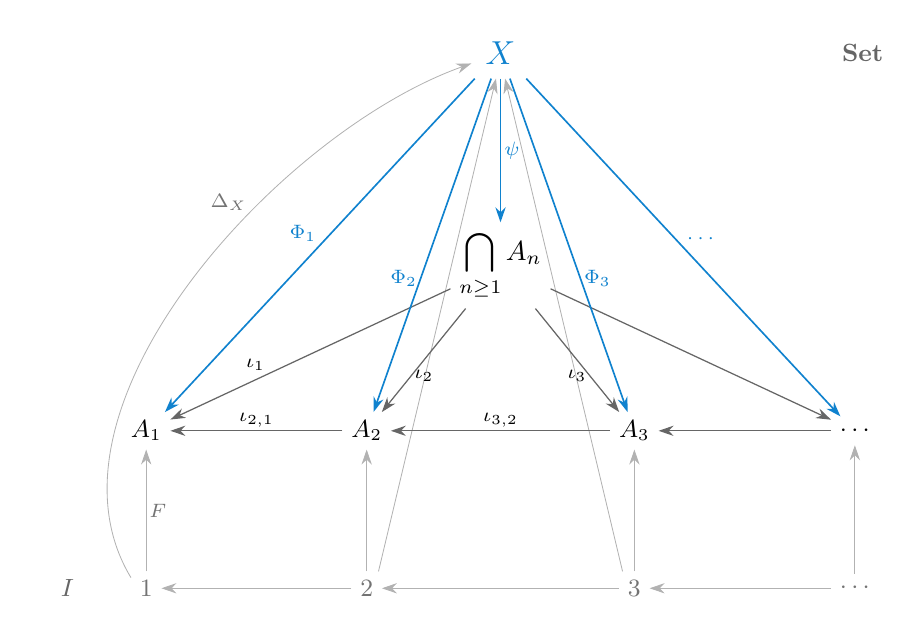
\begin{tikzpicture}[
		>={Stealth[length=1.9mm, width=1.3mm]},
		every node/.style={font=\small},
		object/.style={fill=white, inner sep=3pt},
		correspondence/.style={->, draw=black!30, line width=0.3pt},
		inclusion/.style={->, draw=black!60, line width=0.45pt},
		cone/.style={->, draw=cyan!65!blue, line width=0.6pt},
		maplabel/.style={font=\scriptsize, inner sep=1pt}
	]
		\node[object, font=\large, inner sep=5pt, text=cyan!65!blue] (X) at (0,4.8) {$X$};
		\node[object, font=\normalsize] (A) at (0,2.1) {$\displaystyle\bigcap_{n\ge1}A_n$};
		\node[object] (Aone) at (-4.5,0) {$A_1$};
		\node[object] (Atwo) at (-1.7,0) {$A_2$};
		\node[object] (Athree) at (1.7,0) {$A_3$};
		\node[object] (Adots) at (4.5,0) {$\cdots$};
		\node[object, text=black!55] (one) at (-4.5,-2) {$1$};
		\node[object, text=black!55] (two) at (-1.7,-2) {$2$};
		\node[object, text=black!55] (three) at (1.7,-2) {$3$};
		\node[object, text=black!55] (idots) at (4.5,-2) {$\cdots$};
		\node[text=black!60] at (-5.5,-2) {$I$};
		\node[text=black!60] at (4.6,4.8) {$\mathbf{Set}$};

		\draw[correspondence] (two) -- (one);
		\draw[correspondence] (three) -- (two);
		\draw[correspondence] (idots) -- (three);
		\draw[correspondence] (one) -- node[maplabel, right, text=black!55] {$F$} (Aone);
		\draw[correspondence] (two) -- (Atwo);
		\draw[correspondence] (three) -- (Athree);
		\draw[correspondence] (idots) -- (Adots);
		\draw[correspondence] (one.145) .. controls (-6,0.3) and (-2.8,3.8) ..
			node[maplabel, pos=0.62, above left, text=black!55] {$\Delta_X$} (X.200);
		\draw[correspondence] (two.55) -- (X.260);
		\draw[correspondence] (three.125) -- (X.280);

		\draw[inclusion] (Atwo) -- node[maplabel, above] {$\iota_{2,1}$} (Aone);
		\draw[inclusion] (Athree) -- node[maplabel, above] {$\iota_{3,2}$} (Atwo);
		\draw[inclusion] (Adots) -- (Athree);
		\draw[inclusion] (A) -- node[maplabel, pos=0.65, above left] {$\iota_1$} (Aone);
		\draw[inclusion] (A) -- node[maplabel, pos=0.65, right] {$\iota_2$} (Atwo);
		\draw[inclusion] (A) -- node[maplabel, pos=0.65, left] {$\iota_3$} (Athree);
		\draw[inclusion] (A) -- (Adots);

		\draw[cone] (X.225) --
			node[maplabel, pos=0.5, above left, text=cyan!65!blue] {$\Phi_1$} (Aone.45);
		\draw[cone] (X.250) --
			node[maplabel, pos=0.6, left, text=cyan!65!blue] {$\Phi_2$} (Atwo.70);
		\draw[cone] (X.290) --
			node[maplabel, pos=0.6, right, text=cyan!65!blue] {$\Phi_3$} (Athree.110);
		\draw[cone] (X.315) --
			node[maplabel, pos=0.5, above right, text=cyan!65!blue] {$\cdots$} (Adots.135);
		\draw[cone, line width=0.7pt] (X) --
			node[maplabel, right, text=cyan!65!blue] {$\psi$} (A);
	\end{tikzpicture}
	\end{center}

	\paragraph{(b)} 根据定义, 显然有 $a_N \le a_{N+1}$, $b_N \ge b_{N+1}$, 因此 $I_N \supset I_{N+1}$. 由于原数列有界, 两列 $\{a_N\}$, $\{b_N\}$ 也均有界. 根据单调有界数列的收敛定理, 有 $a = \sup_{N\ge 1} a_N = \lim_{N \to \infty} a_N$, 同理 $b = \lim_{N \to \infty} b_N$. 由于 $a_N \le b_N$, 取极限知 $a \le b$. 并且, 对于任意的 $x\in\R$, 有
	\[ x\in\bigcap_{N\ge1} I_N \Longleftrightarrow \forall\,N\ge1,\ a_N\le x\le b_N \Longleftrightarrow a\le x\le b. \]
	因此 $\bigcap_{N\ge1} I_N = [a,b]$. 直接使用 \textbf{(a)} 的结论, 可知 $\lim(I_1 \leftarrow I_2 \leftarrow \dots) \cong [a, b]$.

	\paragraph{(c)} 事实上, 
	\[ \{x_n\} \text{ 收敛 } \Longleftrightarrow \limsup_{n \to \infty} x_n = \liminf_{n \to \infty} x_n \Longleftrightarrow a = b. \]
	若 $x_n\to l$, 则对任意的 $\varepsilon>0$, 当 $N$ 充分大时有 $l-\varepsilon\le a_N\le b_N\le l+\varepsilon$, 取极限并由 $\varepsilon$ 的任意性知 $a=b=l$. 反之, 若 $a=b=l$, 则由 $a_N,b_N\to l$ 及 $a_N\le x_n\le b_N$ ($n\ge N$), 知 $x_n\to l$.
	此时, $\{x_n\}$ 的上极限和下极限均与极限相等. 当 $x_n = (-1)^{n}$ 时, 极限为 $[-1, 1]$. 
\end{solution}



\begin{problem}
({\heiti 选做}) 记 $\mathbf{Top}$ 为拓扑空间与连续映射组成的范畴. 一个拓扑称为离散拓扑 (discrete topology), 若每个子集都是开集. 令
\[
  S=\{0\}\cup\{1/n:n\ge1\}\subseteq\R,\qquad S_N=\{0\}\cup\{1/n:1\le n\le N\},
\]
并赋予它们由 $\R$ 的通常拓扑诱导的子空间拓扑. 考虑包含映射组成的图 $S_1\hookrightarrow S_2\hookrightarrow\cdots$.
\begin{enumerate}
  \item[(a)] 证明每个 $S_N$ 都是离散空间. 记 $S_{\mathrm{disc}}$ 为 $S$ 的底层集合赋予离散拓扑所得的空间. 证明 $S_{\mathrm{disc}}$ 连同各包含映射 $S_N\hookrightarrow S_{\mathrm{disc}}$, 是上述图在 $\mathbf{Top}$ 中的余极限.
  \item[(b)] 包含映射 $S_N\hookrightarrow S$ 诱导典范连续映射 $S_{\mathrm{disc}}\to S$. 写出这一映射, 并证明它是双射, 但不是同胚. 由此说明, $S$ 连同给定的包含映射及其通常子空间拓扑, 不是上述图在 $\mathbf{Top}$ 中的余极限.
  \item[(c)] 设 $(x_n)$ 为任意实数列, $\ell\in\R$. 对具有通常子空间拓扑的 $S$, 定义
  \[
    f:S\longrightarrow\R,\qquad f(0)=\ell,\qquad f(1/n)=x_n.
  \]
  证明 $f$ 连续, 当且仅当 $x_n\to\ell$.
\end{enumerate}
\end{problem}

\begin{solution}
	\paragraph{(a)} 由于每一个 $S_N$ 均为具有 $N+1$ 个点的有限集合, 显然可以被 $\R$ 中 $N+1$ 个不交的开集覆盖, 根据子空间拓扑的定义, $S_N$ 中的每一个单点集均为开集, 因而 $S_N$ 为离散空间.

	下面来证明 $S_{\mathrm{disc}}$ 连同 $S_N \hookrightarrow S_{\mathrm{disc}}$ 是上述图在 $\mathbf{Top}$ 中的余极限. 取 $I = \mathcal C_{(\Z_+,\le)}$, 并令 $F(N) = S_N$, $F(M\to N) = \iota_{M,N}$ ($M\le N$), 其中 $\iota_{M,N}: S_M \hookrightarrow S_N$ 是包含映射. 再记 $\iota_N: S_N \hookrightarrow S_{\mathrm{disc}}$, 显然有 $\iota_N\circ\iota_{M,N} = \iota_M$.

	对于任意的拓扑空间 $T$ 与自然变换 $\Phi: F \Longrightarrow \Delta_T$, 其对应的连续映射 $\Phi_N: S_N \to T$ 满足交换关系 $\Phi_M = \Phi_N \circ \iota_{M, N}$. 考虑映射
	\[ \psi : \ S_{\mathrm{disc}} \to T, \ x \mapsto \Phi_N(x)\ (x \in S_N). \]
	对于 $x \in S_M \subset S_N$, 有 $\Phi_M (x) = \Phi_N \circ \iota_{M, N}(x) = \Phi_N (x)$, 因此 $\psi$ 是良定义的. 根据定义, $\psi$ 显然满足交换关系 $\Phi_N = \psi \circ \iota_N$. 由于 $S_{\mathrm{disc}}$ 带有离散拓扑, 其出发的任意映射都是连续的, 因此 $\psi$ 也是连续映射. 并且, 若存在 $\psi_1$, $\psi_2$ 同时满足交换条件, 则对任意的 $x \in S_{\mathrm{disc}}$, 总存在 $N$ 使得 $x \in S_N$, 则
	\[ \psi_1(x) = \psi_1 \circ \iota_N(x) = \Phi_N(x) = \psi_2 \circ \iota_N(x) = \psi_2(x). \]
	因此满足交换条件的 $\psi$ 是唯一的. 从而命题得证.

	\paragraph{(b)} 此映射即为 $f: S_{\mathrm{disc}} \to S, x \mapsto x$. 其显然为双射并连续 (因为 $S_{\mathrm{disc}}$ 是离散空间). 但是其逆映射不是连续的, 因为 $\{0\}$ 在 $S_{\mathrm{disc}}$ 中是开集, 但是其在 $f^{-1}$ 下的原像 $\{0\}$ 在 $S$ 中不是开集. 因此 $S$ 连同对应的包含映射不是余极限.

	\paragraph{(c)} 若 $f$ 连续, 则对 $S$ 中的收敛序列 $\{1/n\} \to 0$, 其像在 $\R$ 中也收敛, 即 $\{f(1/n)\} \to f(0)$, 即 $\lim_{n \to \infty} x_n = \ell$. 反之, 若 $x_n \to \ell$, 则对任意的序列 $\{m_n\} \subset S$, 若 $\{m_n\}$ 收敛, 则要么 $m_n \to 0$, 要么 $\{m_n\}$ 在有限项之后的所有项均相同. 在第一种情况下, 非零项 $m_n = 1/k_n$ 的分母最终超过任意给定的正整数, 而零项的像恒为 $\ell$, 因此 $f(m_n)\to\ell=f(0)$; 在第二种情况下, 显然有 $f(m_n)\to f(\lim m_n)$. 由于 $S$ 是度量空间, 因此根据序列判据知 $f$ 连续.
\end{solution}



\begin{problem}
({\heiti 选做}) 设 $I,J$ 为小范畴, $\mathcal C$ 中所有以 $I$ 为指标的图及所有以 $J$ 为指标的图都存在极限. 设 $F:I\times J\to\mathcal C$ 为函子. 乘积范畴 $I\times J$ 的对象为 $(i,j)$, 从 $(i,j)$ 到 $(i',j')$ 的态射为 $(\alpha,\beta)$, 其中 $\alpha:i\to i'$, $\beta:j\to j'$, 复合逐个分量进行.
\begin{enumerate}
  \item[(a)] 对每个 $i\in\operatorname{Ob}(I)$, 选择极限
  \[
    L_i=\lim_{j\in J}F(i,j),\qquad p_{i,j}:L_i\to F(i,j).
  \]
  对态射 $\alpha:i\to i'$, 利用泛性质构造唯一态射 $L(\alpha):L_i\to L_{i'}$, 满足
  \[
    p_{i',j}\circ L(\alpha)=F(\alpha,\operatorname{id}_j)\circ p_{i,j}\qquad\text{对所有 }j\in\operatorname{Ob}(J).
  \]
  证明这些态射使 $i\mapsto L_i$ 成为函子 $L:I\to\mathcal C$.
  \item[(b)] 取 $M=\lim_{i\in I}L_i$, 记其结构映射为 $m_i:M\to L_i$. 证明 $M$ 连同态射族 $r_{i,j}=p_{i,j}\circ m_i:M\to F(i,j)$, 是 $F$ 的极限. 具体地, 先验证对每个态射 $(\alpha,\beta):(i,j)\to(i',j')$ 都有
  \[
    F(\alpha,\beta)\circ r_{i,j}=r_{i',j'}.
  \]
  再证明: 对任意对象 $T$ 及对所有上述态射均满足 $F(\alpha,\beta)\circ t_{i,j}=t_{i',j'}$ 的态射族 $t_{i,j}:T\to F(i,j)$, 存在唯一态射 $t:T\to M$, 使 $r_{i,j}\circ t=t_{i,j}$ 对所有 $(i,j)$ 成立.
  \item[(c)] 由此证明, 以 $I\times J$ 为指标的图 $F$ 存在极限, 且有典范同构
  \begin{gather*}
    \lim_{i\in I}\left(\lim_{j\in J}F(i,j)\right)\cong\lim_{(i,j)\in I\times J}F(i,j) 
    \cong\lim_{j\in J}\left(\lim_{i\in I}F(i,j)\right).
  \end{gather*}
  说明这些同构与各极限到 $F(i,j)$ 的结构映射如何相容.
\end{enumerate}
提示: 第 (b) 问对每个固定的 $i$, 先将态射族 $t_{i,j}$ 通过 $L_i$ 分解, 得到 $u_i:T\to L_i$; 再利用唯一性证明 $L(\alpha)\circ u_i=u_{i'}$, 最后使用 $M$ 的泛性质.
\end{problem}

\begin{solution}
	\paragraph{(a)} 固定 $i, i' \in \Obj(I)$ 和态射 $\alpha: i \to i'$. 构造 $\mathcal{C}$ 中的态射 $\Phi_j = F(\alpha, \id_j) \circ p_{i, j}: L_i \to F(i', j)$.

	先来验证所构造的 $\Phi_j$ 可以看做自然变换 $\Phi: \Delta_{L_i} \Longrightarrow F(i', \cdot)$, 其中这两个函子均从范畴 $J$ 出发. 对于任意的态射 $\beta: j \to j'$, 只需验证 $\Phi_{j'} = F(\id_{i'}, \beta) \circ \Phi_j$. 事实上, 由于 $p_{i,j}$ 是极限锥的结构映射, 有 $p_{i,j'} = F(\id_i, \beta) \circ p_{i,j}$. 再结合 $F$ 是函子, 知
	\begin{align*}
		F(\id_{i'}, \beta) \circ \Phi_j
		&= F(\id_{i'}, \beta) \circ F(\alpha, \id_j) \circ p_{i,j} \\
		&= F(\alpha, \beta) \circ p_{i,j} \\
		&= F(\alpha, \id_{j'}) \circ F(\id_i, \beta) \circ p_{i,j} \\
		&= F(\alpha, \id_{j'}) \circ p_{i,j'} = \Phi_{j'}.
	\end{align*}
	因此 $\Phi$ 满足自然变换所要求的交换条件.

	再用泛性质构造 $L(\alpha)$. 由于 $L_{i'}$ 连同 $p_{i',j}$ 是 $F(i', \cdot)$ 的极限, 而 $\Phi$ 给出了以 $L_i$ 为顶点的锥, 因此存在唯一的态射 $L(\alpha): L_i \to L_{i'}$, 使得对于所有的 $j \in \Obj(J)$, 均有
	\[ p_{i',j} \circ L(\alpha) = \Phi_j = F(\alpha, \id_j) \circ p_{i,j}. \]
	\begin{center}
	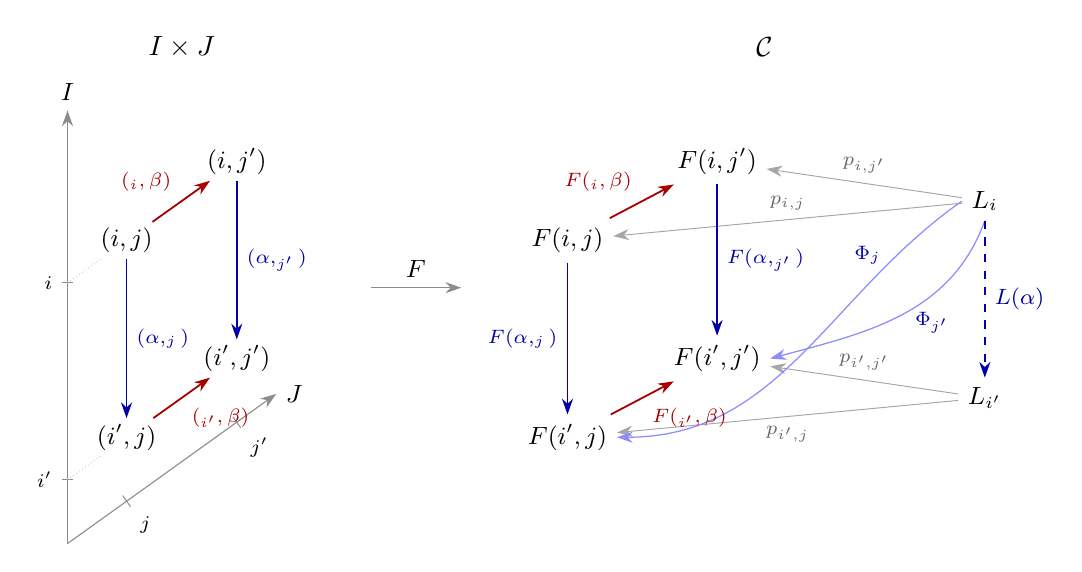
\begin{tikzpicture}[
		>={Stealth[length=2mm, width=1.4mm]},
		every node/.style={font=\small},
		projection/.style={->, draw=black!35, line width=0.35pt},
		cone/.style={->, draw=blue!45, line width=0.45pt},
		alongi/.style={->, blue!65!black, line width=0.65pt},
		alongj/.style={->, red!65!black, line width=0.65pt}
	]
		\node[font=\normalsize] at (0.7,3.65) {$I\times J$};
		\node[font=\normalsize] at (8.1,3.65) {$\mathcal C$};

			\coordinate (origin) at (-0.75,-2.65);
			\draw[->, draw=black!45, line width=0.4pt] (origin) -- (-0.75,2.85)
			node[above, text=black] {$I$};
			\draw[draw=black!45, line width=0.35pt] (-0.82,0.66) -- (-0.68,0.66);
			\node[left, font=\scriptsize] at (-0.82,0.66) {$i$};
			\draw[draw=black!45, line width=0.35pt] (-0.82,-1.84) -- (-0.68,-1.84);
			\node[left, font=\scriptsize] at (-0.82,-1.84) {$i'$};
			\draw[densely dotted, draw=black!25, line width=0.3pt] (-0.75,0.66) -- (0,1.2);
			\draw[densely dotted, draw=black!25, line width=0.3pt] (-0.75,-1.84) -- (0,-1.3);
			\draw[->, draw=black!45, line width=0.4pt] (origin) -- (1.9,-0.75)
			node[right, text=black] {$J$};
			\draw[draw=black!45, line width=0.35pt] (-0.05,-2.04) -- (0.05,-2.18)
				node[below right, font=\scriptsize, text=black] {$j$};
			\draw[draw=black!45, line width=0.35pt] (1.35,-1.04) -- (1.45,-1.18)
			node[below right, font=\scriptsize, text=black] {$j'$};

		\node[fill=white, inner sep=2pt] (ij) at (0,1.2) {$(i,j)$};
		\node[fill=white, inner sep=2pt] (ijprime) at (1.4,2.2) {$(i,j')$};
		\node[fill=white, inner sep=2pt] (iprimej) at (0,-1.3) {$(i',j)$};
		\node[fill=white, inner sep=2pt] (iprimejprime) at (1.4,-0.3) {$(i',j')$};
			\draw[alongi] (ij) -- node[right, font=\scriptsize] {$(\alpha,\id_j)$} (iprimej);
		\draw[alongi] (ijprime) -- node[right, font=\scriptsize] {$(\alpha,\id_{j'})$} (iprimejprime);
		\draw[alongj] (ij) -- node[above left, font=\scriptsize] {$(\id_i,\beta)$} (ijprime);
		\draw[alongj] (iprimej) -- node[below right, font=\scriptsize] {$(\id_{i'},\beta)$} (iprimejprime);

		\draw[->, draw=black!45, line width=0.45pt] (3.1,0.6) --
			node[above, text=black] {$F$} (4.25,0.6);

		\node (Fij) at (5.6,1.2) {$F(i,j)$};
		\node (Fijprime) at (7.5,2.2) {$F(i,j')$};
		\node (Fiprimej) at (5.6,-1.3) {$F(i',j)$};
		\node (Fiprimejprime) at (7.5,-0.3) {$F(i',j')$};
			\node (Li) at (10.9,1.7) {$L_i$};
			\node (Liprime) at (10.9,-0.8) {$L_{i'}$};

		\draw[projection] (Li) -- node[above, text=black!60, font=\scriptsize] {$p_{i,j}$} (Fij);
		\draw[projection] (Li) -- node[above, text=black!60, font=\scriptsize] {$p_{i,j'}$} (Fijprime);
		\draw[projection] (Liprime) -- node[below, text=black!60, font=\scriptsize] {$p_{i',j}$} (Fiprimej);
		\draw[projection] (Liprime) -- node[above, text=black!60, font=\scriptsize] {$p_{i',j'}$} (Fiprimejprime);
			\draw[cone] (Li.west) to[out=-145,in=0]
				node[pos=0.22, above left, text=blue!65!black, font=\scriptsize,
					fill=white, inner sep=1pt] {$\Phi_j$} (Fiprimej.east);
		\draw[cone] (Li.south) to[out=-110,in=15]
			node[pos=0.45, below right, text=blue!65!black, font=\scriptsize,
				fill=white, inner sep=1pt] {$\Phi_{j'}$} (Fiprimejprime.east);

		\draw[alongi] (Fij) -- node[left, font=\scriptsize] {$F(\alpha,\id_j)$} (Fiprimej);
		\draw[alongi] (Fijprime) -- node[right, font=\scriptsize] {$F(\alpha,\id_{j'})$} (Fiprimejprime);
		\draw[alongj] (Fij) -- node[above left, font=\scriptsize] {$F(\id_i,\beta)$} (Fijprime);
		\draw[alongj] (Fiprimej) -- node[below right, font=\scriptsize] {$F(\id_{i'},\beta)$} (Fiprimejprime);
		\draw[alongi, dashed] (Li) -- node[right, font=\footnotesize] {$L(\alpha)$} (Liprime);
	\end{tikzpicture}
	\end{center}

	
	下面来证明所构造的 $L$ 是函子. 对于 $I$ 中的可复合态射 $i \xrightarrow{\alpha} i' \xrightarrow{\alpha'} i''$, 以及任意的 $j \in \Obj(J)$, 根据 $L(\alpha)$ 和 $L(\alpha')$ 的定义, 有
	\begin{align*}
		p_{i'',j} \circ L(\alpha') \circ L(\alpha)
		&= F(\alpha',\id_j) \circ p_{i',j} \circ L(\alpha) \\
		&= F(\alpha',\id_j) \circ F(\alpha,\id_j) \circ p_{i,j} \\
		&= F(\alpha'\circ\alpha,\id_j) \circ p_{i,j} \\
		&= p_{i'',j} \circ L(\alpha'\circ\alpha).
	\end{align*}
	由于上述等式对所有的 $j \in \Obj(J)$ 均成立, 因此根据 $L_{i''}$ 的极限泛性质中的唯一性, 知 $L(\alpha') \circ L(\alpha) = L(\alpha'\circ\alpha)$.

	再来验证 $L$ 保持恒等态射. 对于任意的 $i \in \Obj(I)$ 和 $j \in \Obj(J)$, 有
	\[ p_{i,j} \circ L(\id_i) = F(\id_i,\id_j) \circ p_{i,j} = p_{i,j} = p_{i,j} \circ \id_{L_i}. \]
	同样根据 $L_i$ 的极限泛性质中的唯一性, 知 $L(\id_i) = \id_{L_i}$. 综上, $i \mapsto L_i$, $\alpha \mapsto L(\alpha)$ 给出了函子 $L: I \to \mathcal C$.
	\begin{center}
	\begin{tikzpicture}[
		>={Stealth[length=2mm, width=1.4mm]},
		every node/.style={font=\small},
		projection/.style={->, draw=black!35, line width=0.35pt},
		image/.style={->, draw=black!65, line width=0.55pt},
		induced/.style={->, draw=blue!65!black, line width=0.65pt}
	]
		\node[font=\normalsize] at (0,3.05) {$I$};
		\node[font=\normalsize] at (7.3,3.05) {$\mathcal C$};

		\node (i) at (0,2.2) {$i$};
		\node (iprime) at (0,0) {$i'$};
		\node (iprimeprime) at (0,-2.2) {$i''$};
		\draw[induced] (i) -- node[left, font=\footnotesize] {$\alpha$} (iprime);
		\draw[induced] (iprime) -- node[left, font=\footnotesize] {$\alpha'$} (iprimeprime);
		\draw[->, draw=black!45, line width=0.45pt] (1.3,0.8) --
			node[above, text=black, font=\footnotesize] {$F(-,j)$} (2.8,0.8);

		\node (Fij) at (5,2.2) {$F(i,j)$};
		\node (Fiprimej) at (5,0) {$F(i',j)$};
		\node (Fiprimeprimej) at (5,-2.2) {$F(i'',j)$};
		\node (Li) at (9.3,2.2) {$L_i$};
		\node (Liprime) at (9.3,0) {$L_{i'}$};
		\node (Liprimeprime) at (9.3,-2.2) {$L_{i''}$};

		\draw[projection] (Li) -- node[above, text=black!60, font=\scriptsize] {$p_{i,j}$} (Fij);
		\draw[projection] (Liprime) -- node[above, text=black!60, font=\scriptsize] {$p_{i',j}$} (Fiprimej);
		\draw[projection] (Liprimeprime) -- node[below, text=black!60, font=\scriptsize] {$p_{i'',j}$} (Fiprimeprimej);
		\draw[image] (Fij) -- node[right, font=\scriptsize] {$F(\alpha,\id_j)$} (Fiprimej);
		\draw[image] (Fiprimej) -- node[right, font=\scriptsize] {$F(\alpha',\id_j)$} (Fiprimeprimej);
		\draw[image] (Fij.west) to[out=-135,in=135]
			node[left, font=\scriptsize] {$F(\alpha'\circ\alpha,\id_j)$} (Fiprimeprimej.west);
		\draw[induced] (Li) -- node[right, font=\footnotesize] {$L(\alpha)$} (Liprime);
		\draw[induced] (Liprime) -- node[right, font=\footnotesize] {$L(\alpha')$} (Liprimeprime);
		\draw[induced] (Li.east) to[out=-45,in=45]
			node[right, font=\scriptsize] {$L(\alpha'\circ\alpha)$} (Liprimeprime.east);
	\end{tikzpicture}
	\end{center}

	\paragraph{(b)} 先来验证 $r_{i,j}$ 满足极限锥所要求的交换条件. 对于任意的态射 $\alpha: i \to i'$, $\beta: j \to j'$, 由 $F$ 是函子, 并结合 $p_{i,j}$, $m_i$ 的交换条件, 有
	\begin{align*}
		F(\alpha,\beta) \circ r_{i,j}
		&= F(\alpha,\id_{j'}) \circ F(\id_i,\beta) \circ p_{i,j} \circ m_i \\
		&= F(\alpha,\id_{j'}) \circ p_{i,j'} \circ m_i \\
		&= p_{i',j'} \circ L(\alpha) \circ m_i \\
		&= p_{i',j'} \circ m_{i'} = r_{i',j'}.
	\end{align*}
	因此 $M$ 连同态射族 $r_{i,j}$ 给出了 $F$ 的一个锥.

	再来验证泛性质. 对于任意的对象 $T$ 和满足 $F(\alpha,\beta) \circ t_{i,j} = t_{i',j'}$ 的态射族 $t_{i,j}: T \to F(i,j)$, 固定 $i \in \Obj(I)$. 对任意的态射 $\beta: j \to j'$, 均有 $F(\id_i,\beta) \circ t_{i,j} = t_{i,j'}$. 因此, 根据 $L_i$ 的极限泛性质, 存在唯一的态射 $t_i: T \to L_i$, 满足
	\[ p_{i,j} \circ t_i = t_{i,j} \quad (j \in \Obj(J)). \]
	而对于任意的态射 $\alpha: i \to i'$ 和任意的 $j \in \Obj(J)$, 有
	\begin{align*}
		p_{i',j} \circ L(\alpha) \circ t_i
		&= F(\alpha,\id_j) \circ p_{i,j} \circ t_i \\
		&= F(\alpha,\id_j) \circ t_{i,j} \\
		&= t_{i',j} = p_{i',j} \circ t_{i'}.
	\end{align*}
	根据 $L_{i'}$ 的极限泛性质中的唯一性, 知 $L(\alpha) \circ t_i = t_{i'}$. 因此 $t_i$ 给出了 $L$ 的一个锥. 再根据 $M$ 的极限泛性质, 存在唯一的态射 $t: T \to M$, 满足 $m_i \circ t = t_i$. 此时对于任意的 $(i,j)$, 有
	\[ r_{i,j} \circ t = p_{i,j} \circ m_i \circ t = p_{i,j} \circ t_i = t_{i,j}. \]
	若另有态射 $s: T \to M$ 满足所有的 $r_{i,j} \circ s = t_{i,j}$, 则 $p_{i,j} \circ m_i \circ s = t_{i,j}$, 因而由 $t_i$ 的唯一性知 $m_i \circ s = t_i$. 再由 $M$ 的极限泛性质中的唯一性知 $s = t$. 综上, $M$ 连同态射族 $r_{i,j}$ 是 $F$ 的极限.
	\begin{center}
	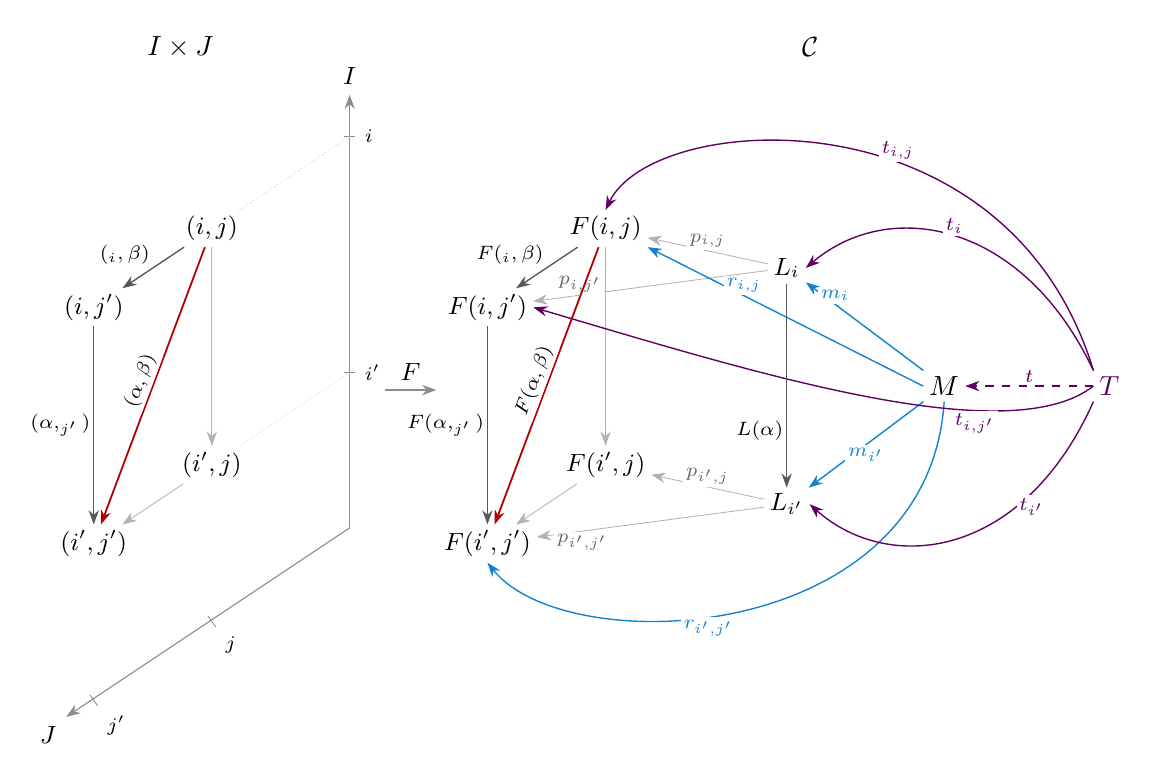
\begin{tikzpicture}[
		>={Stealth[length=1.8mm, width=1.3mm]},
		every node/.style={font=\small},
		object/.style={fill=white, inner sep=2pt},
		auxiliary/.style={->, draw=black!30, line width=0.3pt},
		image/.style={->, draw=black!65, line width=0.5pt},
		composite/.style={->, draw=red!70!black, line width=0.65pt},
		limitmap/.style={->, draw=cyan!65!blue, line width=0.5pt},
		testmap/.style={->, draw=violet!75!black, line width=0.5pt},
		maplabel/.style={font=\scriptsize, fill=white, inner sep=1pt}
	]
		\node[font=\normalsize] at (1.3,4.8) {$I\times J$};
		\node[font=\normalsize] at (9.3,4.8) {$\mathcal C$};
		\coordinate (origin) at (3.45,-1.3);
		\draw[->, draw=black!45, line width=0.4pt] (origin) -- (3.45,4.2)
			node[above, text=black] {$I$};
		\draw[draw=black!45, line width=0.3pt] (3.38,3.67) -- (3.52,3.67)
			node[right, text=black, font=\scriptsize] {$i$};
		\draw[draw=black!45, line width=0.3pt] (3.38,0.67) -- (3.52,0.67)
			node[right, text=black, font=\scriptsize] {$i'$};
		\draw[densely dotted, draw=black!20, line width=0.3pt] (3.45,3.67) -- (1.7,2.5);
		\draw[densely dotted, draw=black!20, line width=0.3pt] (3.45,0.67) -- (1.7,-0.5);
		\draw[->, draw=black!45, line width=0.4pt] (origin) -- (-0.15,-3.7)
			node[below left, text=black] {$J$};
		\draw[draw=black!45, line width=0.3pt] (1.65,-2.42) -- (1.75,-2.56)
			node[below right, text=black, font=\scriptsize] {$j$};
		\draw[draw=black!45, line width=0.3pt] (0.15,-3.42) -- (0.25,-3.56)
			node[below right, text=black, font=\scriptsize] {$j'$};

		\node[object] (ij) at (1.7,2.5) {$(i,j)$};
		\node[object] (ijprime) at (0.2,1.5) {$(i,j')$};
		\node[object] (iprimej) at (1.7,-0.5) {$(i',j)$};
		\node[object] (iprimejprime) at (0.2,-1.5) {$(i',j')$};
		\draw[auxiliary] (ij) -- (iprimej);
		\draw[auxiliary] (iprimej) -- (iprimejprime);
		\draw[image] (ij) -- node[maplabel, above left] {$(\id_i,\beta)$} (ijprime);
		\draw[image] (ijprime) -- node[maplabel, left] {$(\alpha,\id_{j'})$} (iprimejprime);
		\draw[composite] (ij) -- node[maplabel, sloped, above] {$(\alpha,\beta)$} (iprimejprime);
		\draw[->, draw=black!45, line width=0.4pt] (3.9,0.45) --
			node[above, text=black] {$F$} (4.55,0.45);

		\node[object] (Fij) at (6.7,2.5) {$F(i,j)$};
		\node[object] (Fijprime) at (5.2,1.5) {$F(i,j')$};
		\node[object] (Fiprimej) at (6.7,-0.5) {$F(i',j)$};
		\node[object] (Fiprimejprime) at (5.2,-1.5) {$F(i',j')$};
		\node[object] (Li) at (9,2) {$L_i$};
		\node[object] (Liprime) at (9,-1) {$L_{i'}$};
		\node[object, font=\normalsize] (M) at (11,0.5) {$M$};
		\node[object, text=violet!75!black, font=\normalsize] (T) at (13.1,0.5) {$T$};

		\draw[auxiliary] (Li) -- node[maplabel, above, text=black!60] {$p_{i,j}$} (Fij);
		\draw[auxiliary] (Li) -- node[maplabel, pos=0.8, above, text=black!60] {$p_{i,j'}$} (Fijprime);
		\draw[auxiliary] (Liprime) -- node[maplabel, above, text=black!60] {$p_{i',j}$} (Fiprimej);
		\draw[auxiliary] (Liprime) -- node[maplabel, pos=0.8, below, text=black!60] {$p_{i',j'}$} (Fiprimejprime);
		\draw[auxiliary] (Fij) -- (Fiprimej);
		\draw[auxiliary] (Fiprimej) -- (Fiprimejprime);

		\draw[limitmap] (M) -- node[maplabel, pos=0.75, above, text=cyan!65!blue] {$m_i$} (Li);
		\draw[limitmap] (M) -- node[maplabel, below, text=cyan!65!blue] {$m_{i'}$} (Liprime);
		\draw[limitmap] (M.west) -- node[maplabel, pos=0.65, above, text=cyan!65!blue] {$r_{i,j}$} (Fij.south east);
		\draw[limitmap] (M.south) .. controls (10.8,-2.8) and (6.2,-3) ..
			node[maplabel, pos=0.55, below, text=cyan!65!blue] {$r_{i',j'}$} (Fiprimejprime.south);

		\draw[testmap] (T.north west) .. controls (11.8,4.3) and (7.3,4) ..
			node[maplabel, pos=0.4, above, text=violet!75!black] {$t_{i,j}$} (Fij.north);
		\draw[testmap] (T.west) .. controls (11.8,-0.35) and (8.5,0.7) ..
			node[maplabel, pos=0.3, below, text=violet!75!black] {$t_{i,j'}$} (Fijprime.east);
		\draw[testmap] (T.north west) .. controls (12,2.6) and (10.3,2.9) ..
			node[maplabel, above, text=violet!75!black] {$t_i$} (Li.east);
		\draw[testmap] (T.south west) .. controls (12,-1.7) and (10.3,-1.9) ..
			node[maplabel, pos=0.3, right, text=violet!75!black] {$t_{i'}$} (Liprime.east);
		\draw[testmap, dashed, line width=0.65pt] (T) --
			node[maplabel, above, text=violet!75!black] {$t$} (M);

		\draw[image] (Fij) -- node[maplabel, above left] {$F(\id_i,\beta)$} (Fijprime);
		\draw[image] (Fijprime) -- node[maplabel, left] {$F(\alpha,\id_{j'})$} (Fiprimejprime);
		\draw[composite] (Fij) -- node[maplabel, sloped, above] {$F(\alpha,\beta)$} (Fiprimejprime);
		\draw[image] (Li) -- node[maplabel, pos=0.72, left] {$L(\alpha)$} (Liprime);
	\end{tikzpicture}
	\end{center}

	\paragraph{(c)} 由 (b), $M = \lim_{i\in I}(\lim_{j\in J}F(i,j))$ 连同 $r_{i,j}$ 是 $F$ 的极限, 因此以 $I\times J$ 为指标的极限存在. 交换 $I,J$ 的角色, 同理 $N = \lim_{j\in J}(\lim_{i\in I}F(i,j))$ 连同复合投影 $s_{i,j}$ 也是 $F$ 的极限. 记 $P = \lim_{(i,j)\in I\times J}F(i,j)$, 其结构映射为 $q_{i,j}$. 由极限的唯一性, 存在唯一的同构 $\varphi: M \to P$, $\psi: P \to N$, 满足
	\[ q_{i,j} \circ \varphi = r_{i,j}, \qquad s_{i,j} \circ \psi = q_{i,j} \quad ((i,j)\in\Obj(I\times J)). \]
	因此 $M \cong P \cong N$, 即得题目中的同构. 上述等式也说明这些同构与各极限到 $F(i,j)$ 的结构映射相容, 因而是典范同构.
\end{solution}

\end{document}
